\documentclass[12pt]{article}
\usepackage{enumitem}
\usepackage{amsmath}
\usepackage{amssymb}
\usepackage{empheq}
\usepackage{graphicx}
\begin {document}
	\begin{center}
		\large \textbf{A Proposed Implementation of a 16 Bit ALU}
		\normalsize
		\newline \newline
		Arjun Lakshmipathy, ID: 804158733 \\
		Joraaver Chahal, ID: 304200975
	\end{center}
  \section{}

	\textbf{High Level Description:}
	\newline \newline
	Our decided implementation of the bit slice for this 8 bit ALU attempted to target
	minimizing the energy delay product while keeping the overall design as intuitive and 
	readable as possible. Our decided upon implementation was a reasonably modular 
	slice comprised of a combination of simpler gates with varying numbers of inputs. Our
	solution to minimizing the energy product delay of the whole slice was to limit the number
	or transistors used in the circuit. However, in some cases extra transistors were added
	simply to either:
	
	\begin{enumerate}[label=(\alph*)]
		\item Keep the design more readable / maintainable. 
		\newline \newline
		or
		\item Allow a particular component of the circuit to be self-restoring. 
	\end{enumerate}
	These tradeoffs were determined as acceptable since they would simplify some of the
	development process moving forward and would ensure that we did not experience any
	unexpected signal degradation. 
	\newline \newline
	Using this approach, we began constructing some basic gates at the transistor level. The most
	basic gates constructed were the following:
	\begin{itemize}
		\item Inverter
		\item 2-input NAND
		\item 3-input NAND
		\item 2-input NOR
		\item 3-input XOR
		\item Transmission Gate
		\item 2-input MUX
		\item 8-input MUX
		\item 2-output DEMUX
	\end{itemize}
	All other components of the circuit were more or less assembled from these basic building
	blocks. These included:
	\begin{itemize}
		\item 2-input AND
		\item 3-input AND
		\item 2-input OR
		\item Logical Shift (left or right)
		\item Adder
	\end{itemize}
	Finally, using these higher level building blocks, we constructed the "Master" high level
	schematic to serve as our control for the overall slice.Using our master schematic as 
	the control and the components as the actual operations of the ALU, we constructed 
	our overall single bit slice. 
	\newline \newline
	\textbf{More Detailed Breakdowns:}
	\newline \newline
	\textbf{OR-NOR-AND etc. Implementation and Uses:}
	\newline \newline
	Each of these gates was constructed using a static CMOS layout, with the PMOS pull-up 
	network being complementary to the NMOS pull-down network. Each gate was driven by
	its own voltage supply and was connected to ground to ensure that it could drive itself and
	not be dependent on the input. Some of these gates were used as final outputs of the ALU,
	while others were used to build more complex modules or serve as control blocks. The 
	transistors were sized such that both the pull-up and the pull-down network
	both resulted in an ultimate unity resistance, using a base unit of 3$\lambda$. 
	For reference, see some samples below:
	\newline \newline \newline \newline \newline \newline \newline
 	3-input and:\\
  	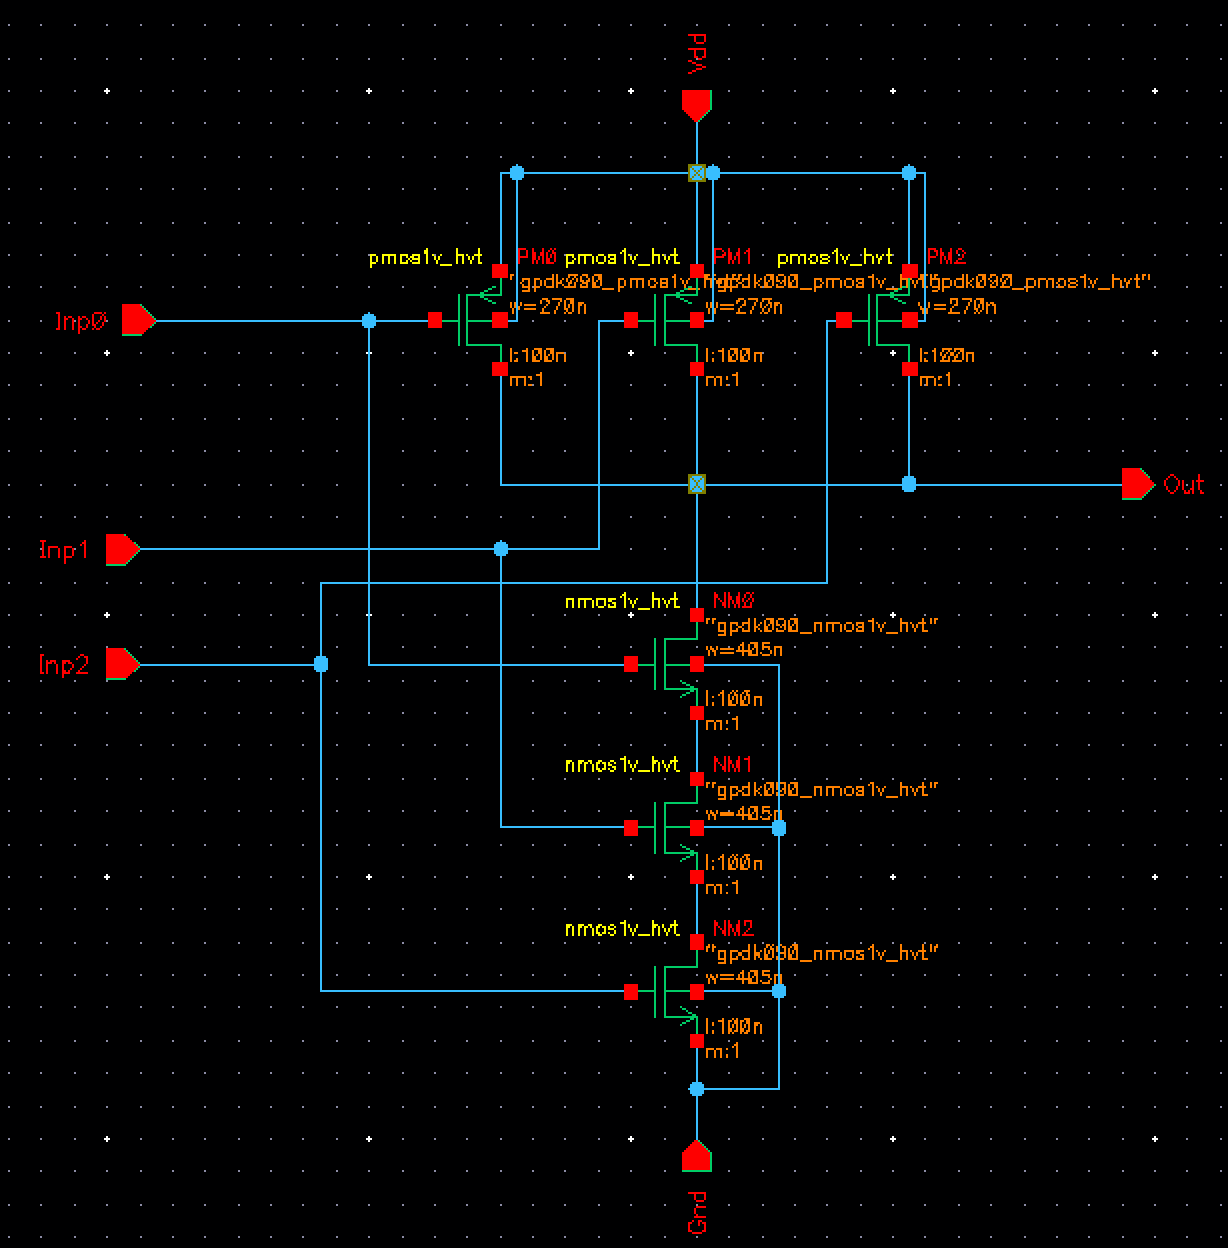
\includegraphics[scale=0.4]{3and.png} \\
	\newline \newline
  	3-input xor:\\
 	 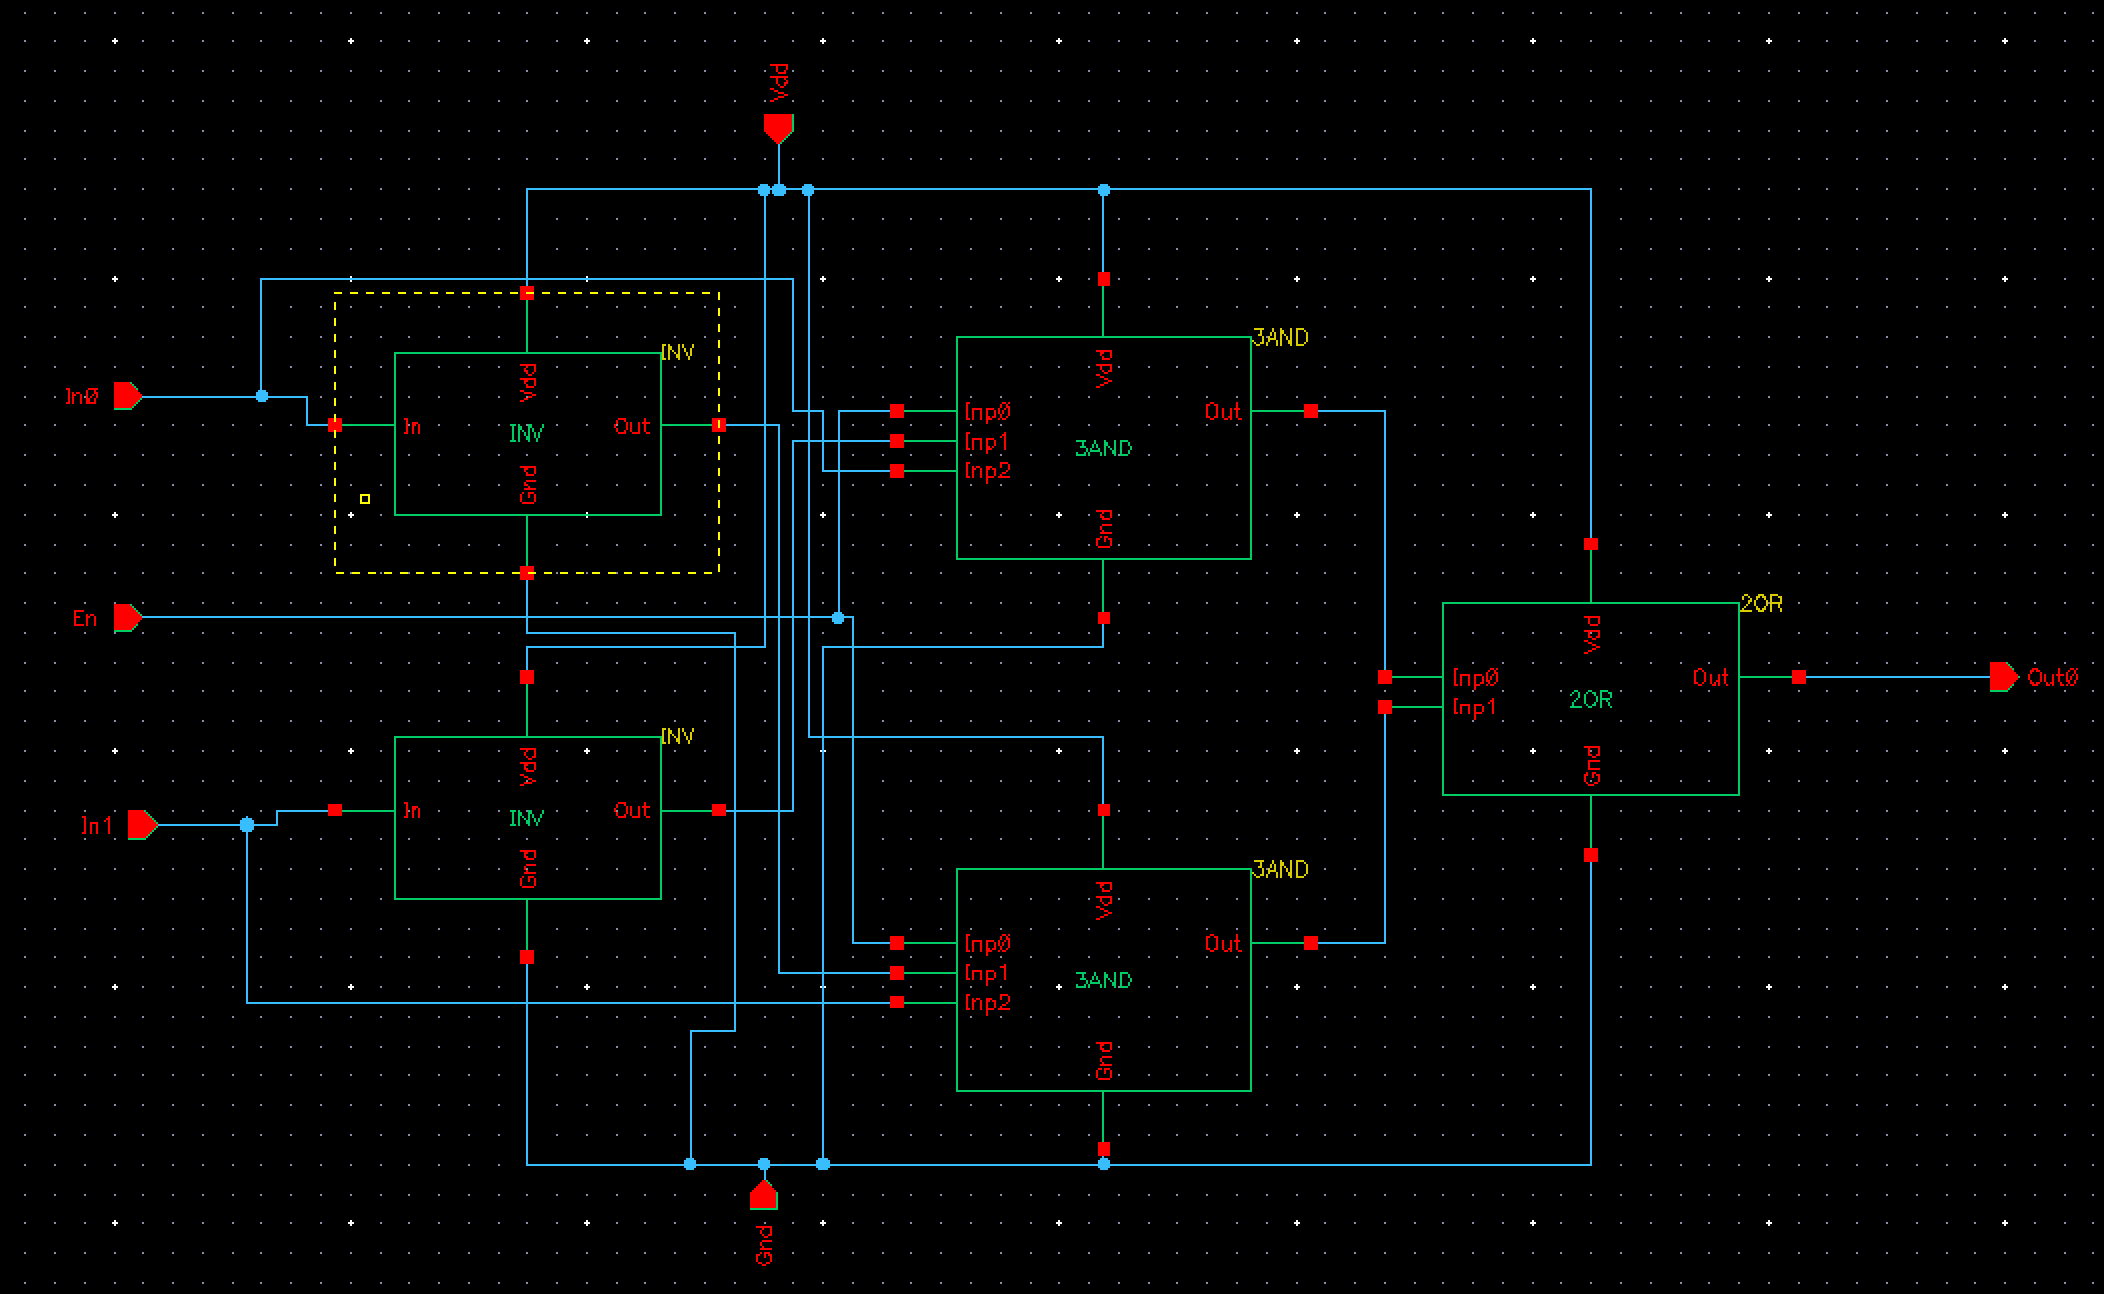
\includegraphics[scale=0.3]{xor.png} \\
	\newline \newline
	\textbf{MUX / DEMUX Implementation and Uses:}
	\newline \newline
	The primary building blocks for each of these gates were transmission gates, with each 
	T-Gate having a 3$\lambda$ NMOS and a 6$\lambda$ PMOS. These gates primarily served
	as control logic for the circuit (our master schematic heavily relies on DEMUX gates), 
	allowing us to handle multiple input modules and granting us the ability to selectively 
	activate only certain portions of the ALU during any particular OpCode
	in order to minimize power consumption. They also served very crucial roles in allowing us to
	compress the left and right shift modules into one by cleverly mapping the input and easily 
	implement the clear operation. The implementation of these gates are pictured below:
	\newline \newline
 	Transmission gate:\\
 	 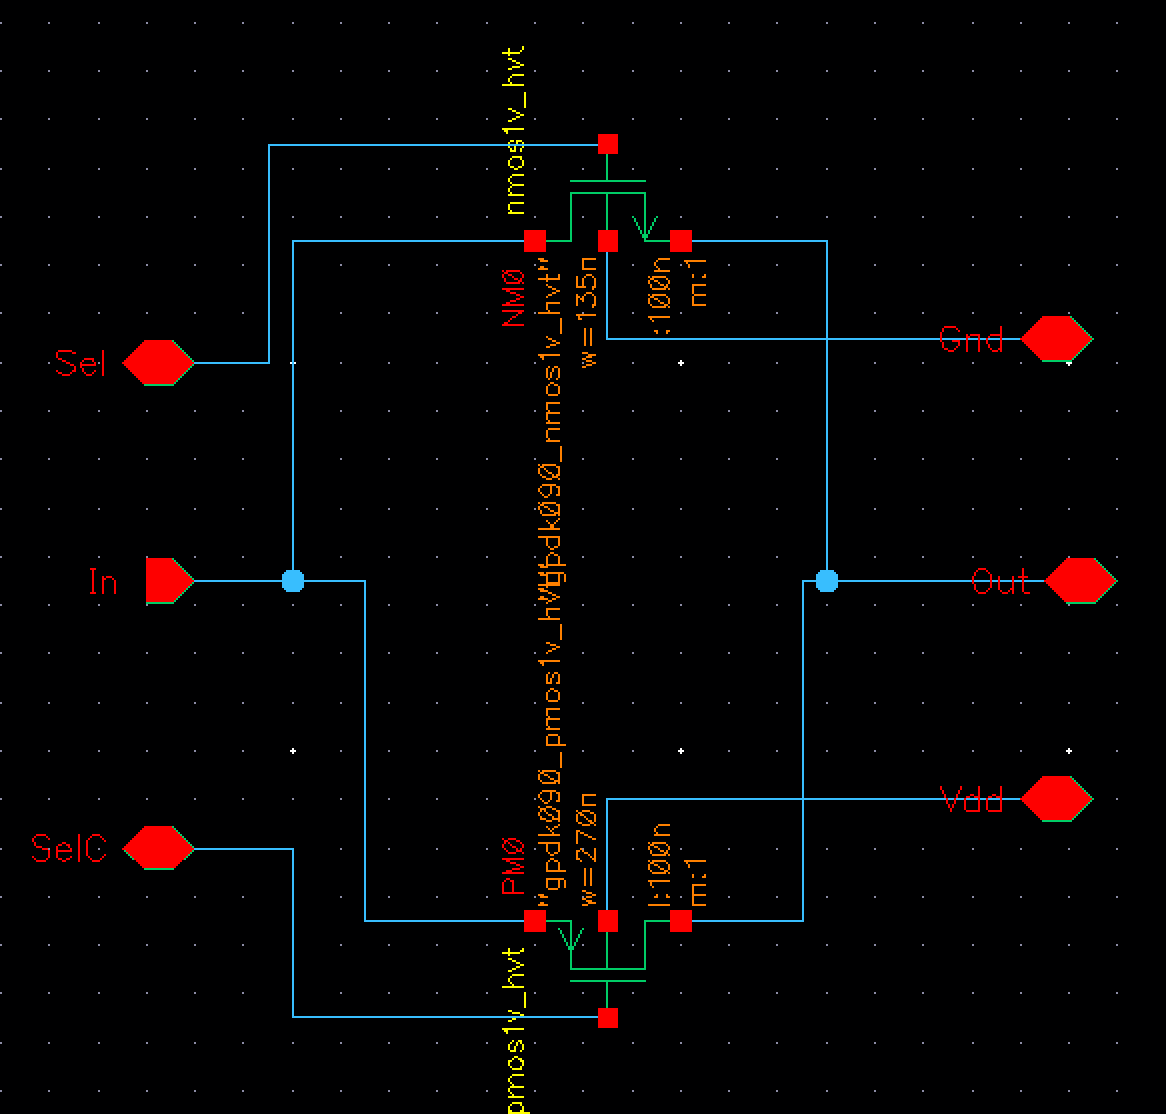
\includegraphics[scale=0.4]{tgate.png} \\
	 \newline \newline \newline \newline \newline \newline \newline \newline
	Shifter:\\
 	 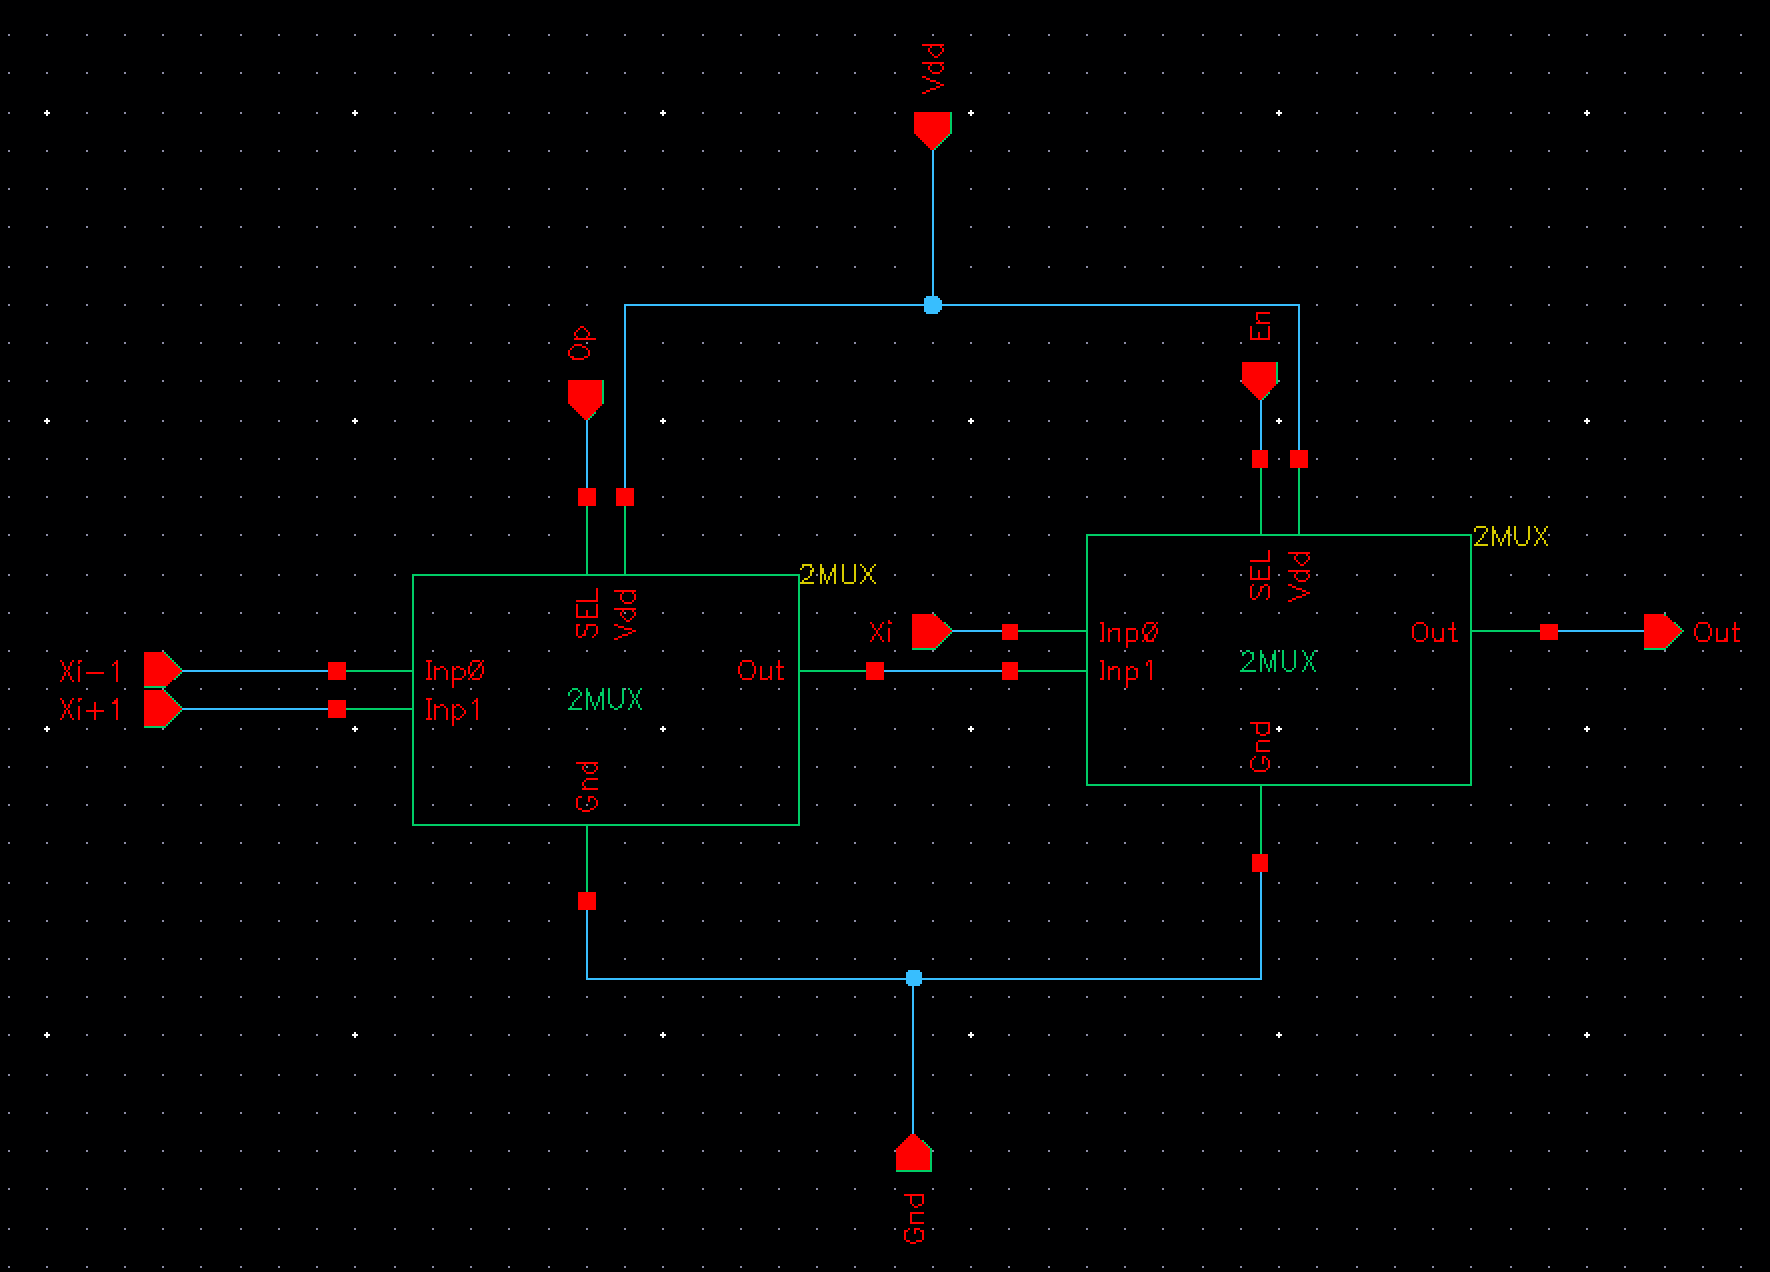
\includegraphics[scale=0.3]{shift.png} \\
	 \newline \newline
	Partial Demux:\\
  	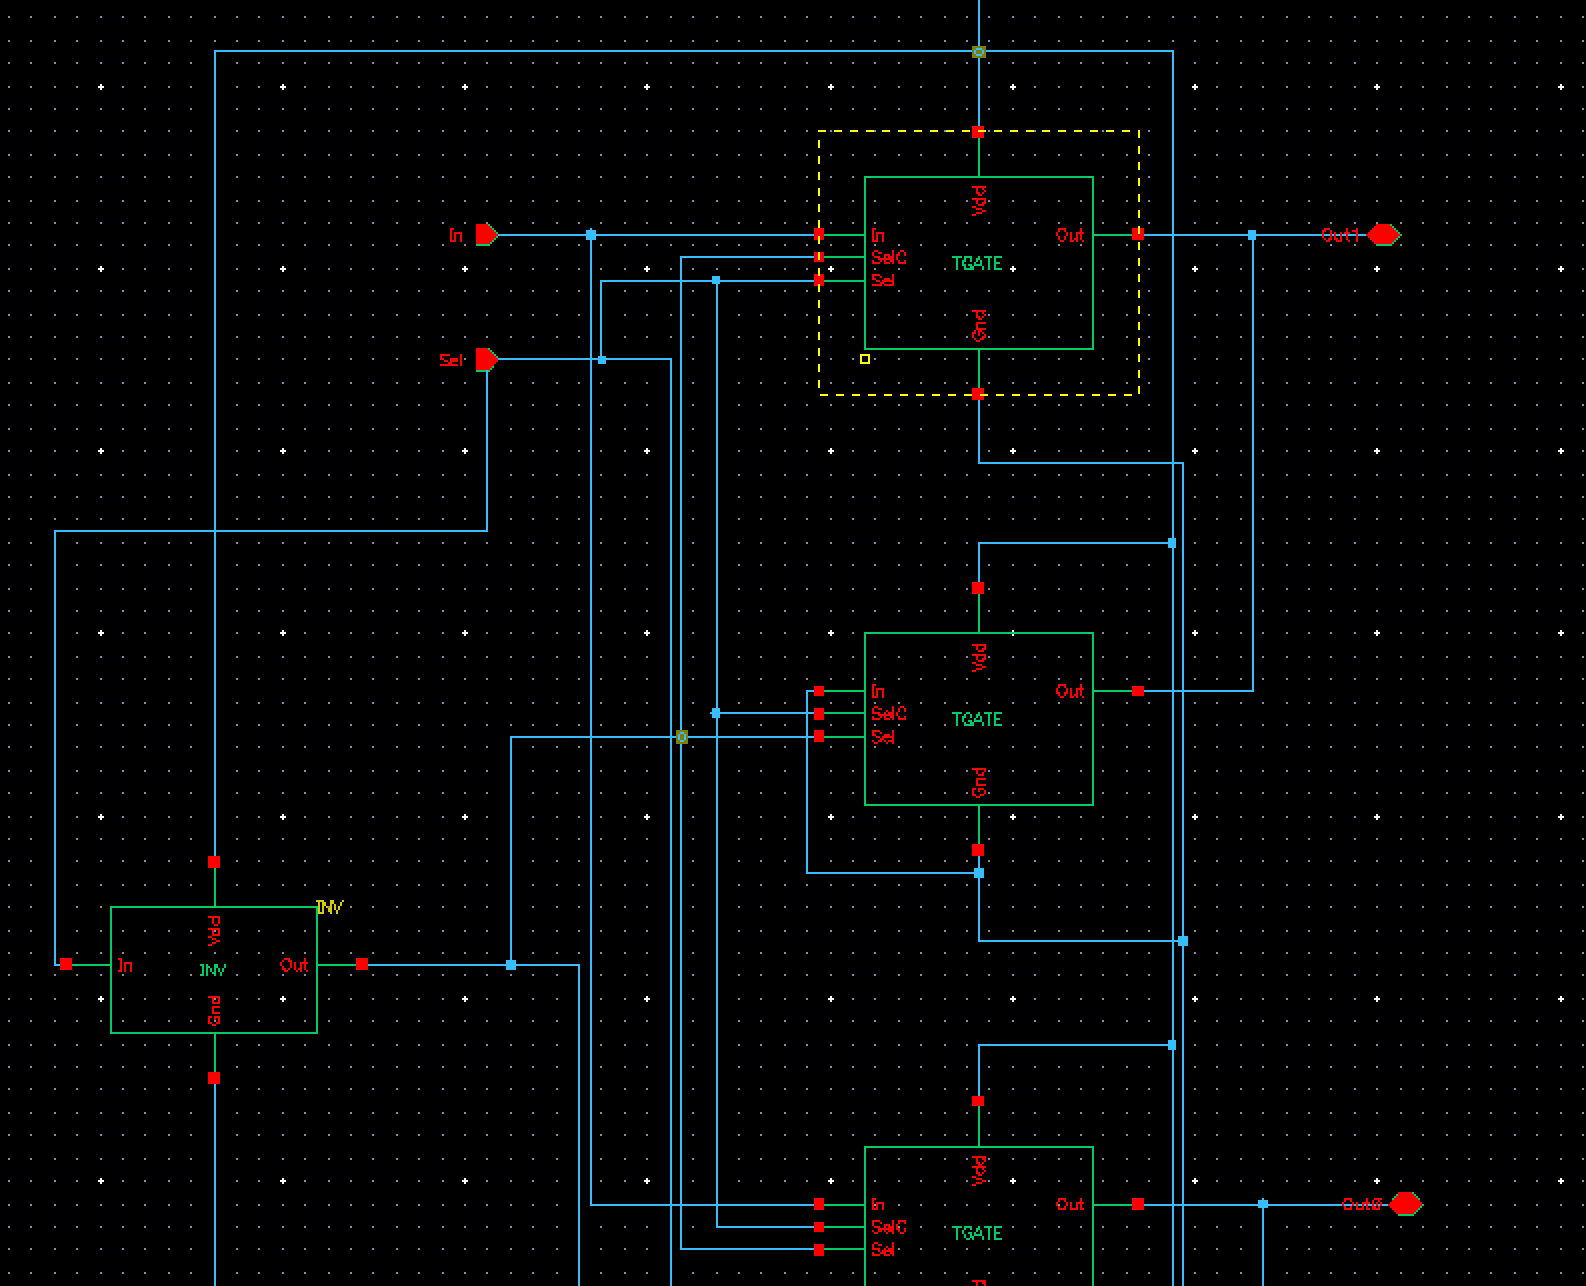
\includegraphics[scale=0.4]{demuxpart.png} \\
	\newline \newline
	A final large 8-input MUX was then used to serve as the final channel to the ultimate output 
	bit for the slice. Though each OpCode is 4 bits in length, we managed to come up with an 
	interesting mapping such that only the 3 least significant bits are used:
	\newline \newline
  	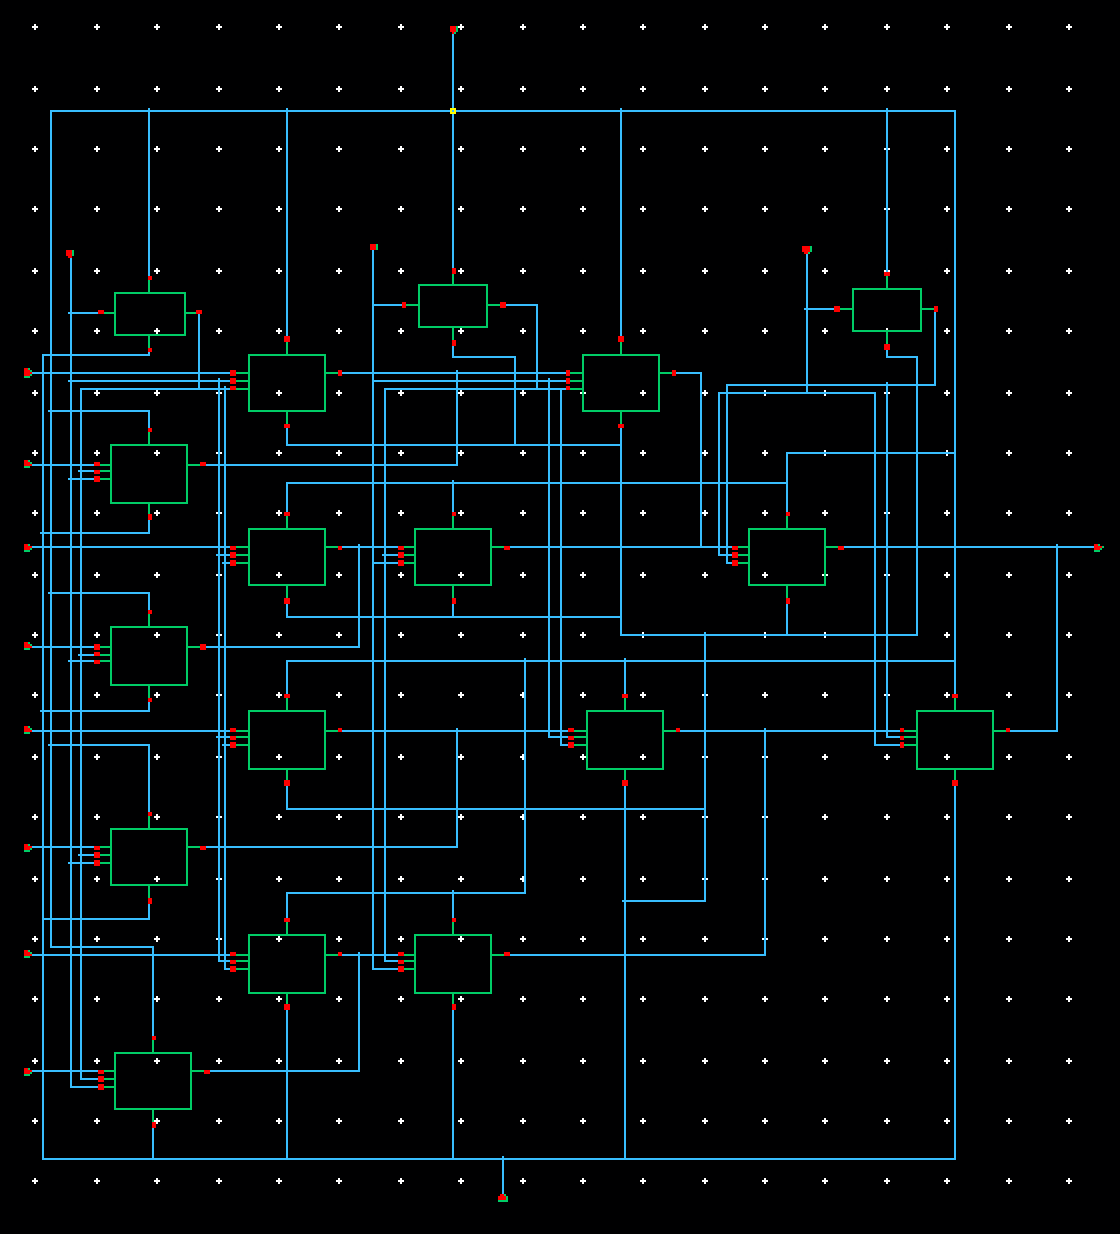
\includegraphics[scale=0.4]{8mux.png} \\
	\newline \newline
	\textbf{Adder Implementation:}
	\newline \newline
	We chose to go with a Carry Look-Ahead adder implementation using a combination of AND,
	OR, and XOR gates, as shown below:
	\newline \newline
 	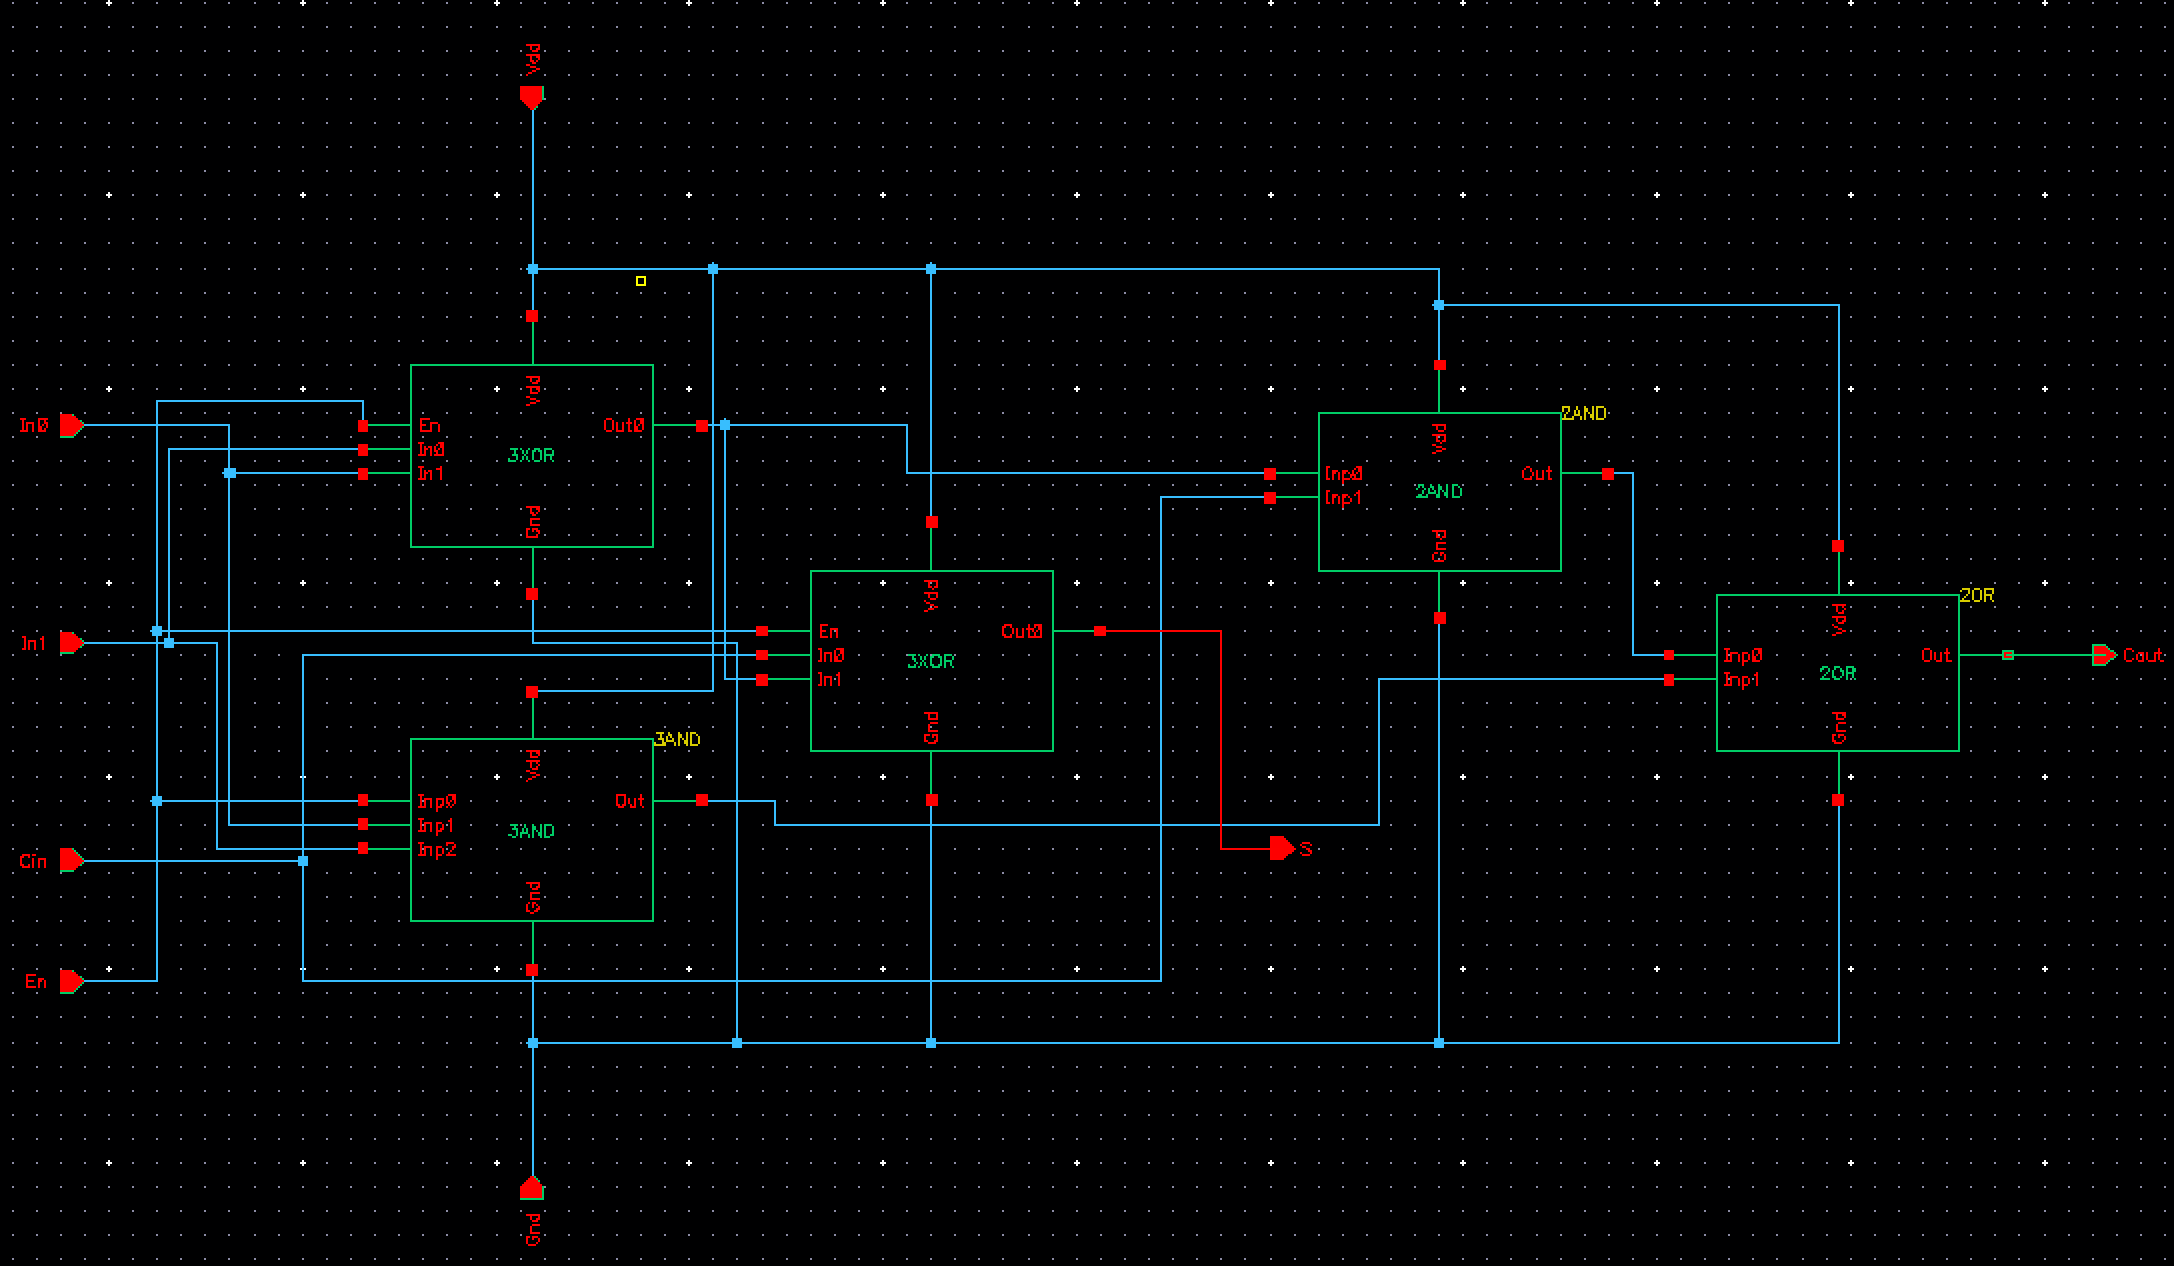
\includegraphics[scale=0.4]{add.png} \\
	\newline \newline
	The Look-Ahead implementation would allow for the parallel computation of the Carry-Out and
	Sum quantities, which would allow us to quickly send the carry-out number on the look-ahead
	bus for other bit slices to absorb. In this regard, we would be significantly reducing the delay
	of the adder module and a reasonable amount of power consumption as well. This minimization
	is further supported by the fact that the adder does not even activate unless the enable bit
	is activated (controlled via a combination of DEMUX gates). Future iterations of the project 
	may include changing this implementation, but for now the attempt seemed good enough to
	suffice.
	\newline \newline
	\textbf{Ending Remarks:}
	\newline \newline
	All components were tested individually for correct functionality before being incorporated 
	into other blocks of the circuit.
	\newline \newline
	
  	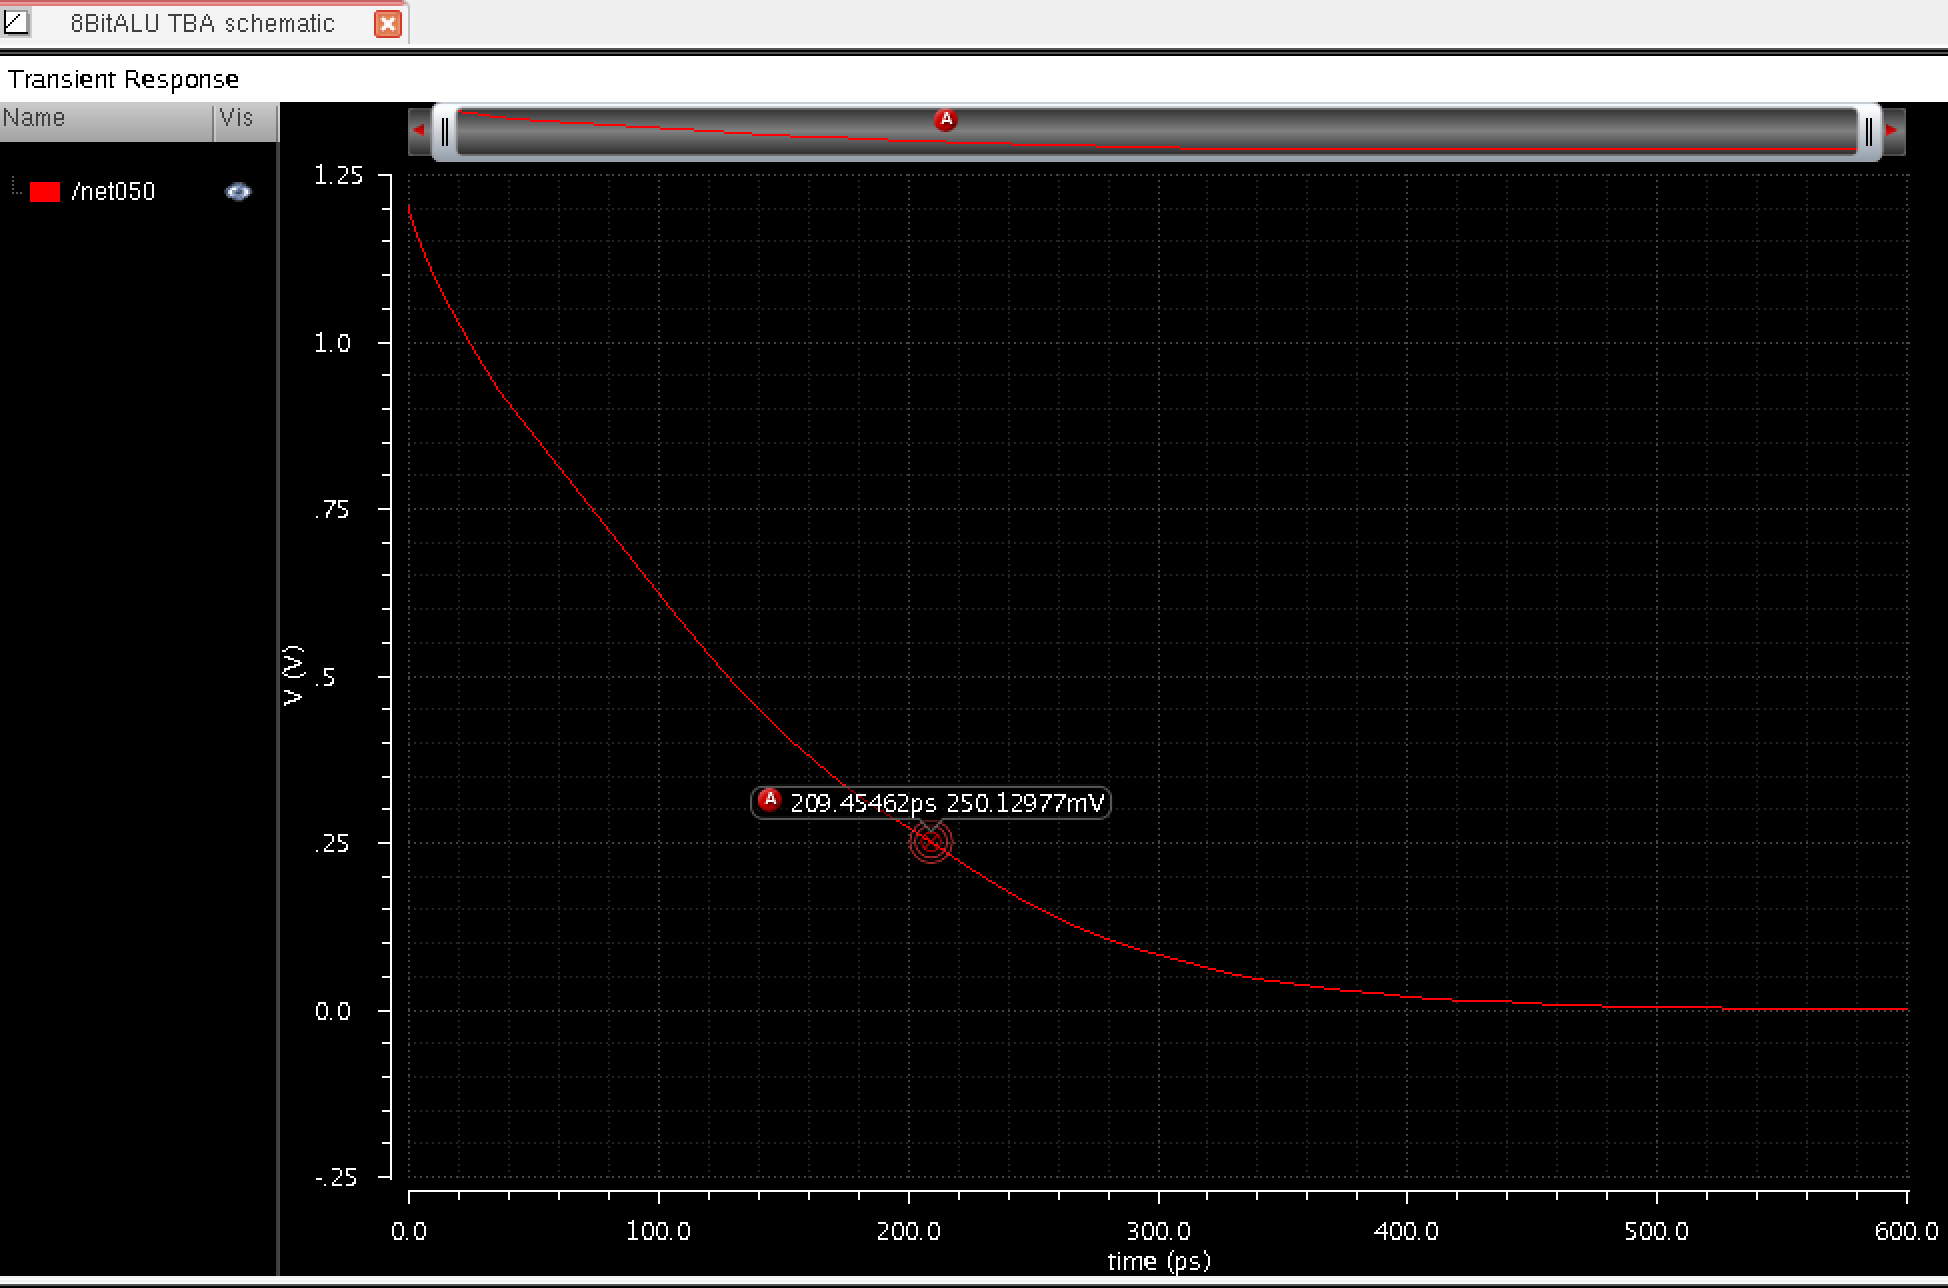
\includegraphics[scale=0.4]{AndDelay.png} \\
	\newline \newline
  	This demonstrates the delay from the Bitwise AND instruction in the ALU. While not the worst 
	delay path in the ALU, it does a reasonable approximation of the work that must be done, since 
	it travels along the farthest path (besides adder instructions). The propagation delay
	here is about 209 ps.
	\newline \newline
	After trying a variety of OpCodes, we found that the slice worked as far as functionality 
	is concerned. For this stage of the project, this was a reasonable testament of our progress
	and hard work.
  \section{}
	
  \textbf{Layouts}
  \newline \newline
  The layouts werw a semi-complicated beast. Once we got the hang of creating the module layouts
  and have them be in the larger circuits, the process got easier. However, every time an LVS failed
  somewhere lower down, each higher circuit needed to be redone to accomadate for said changes.
  \newline \newline
  The master layout:
  \newline \newline
  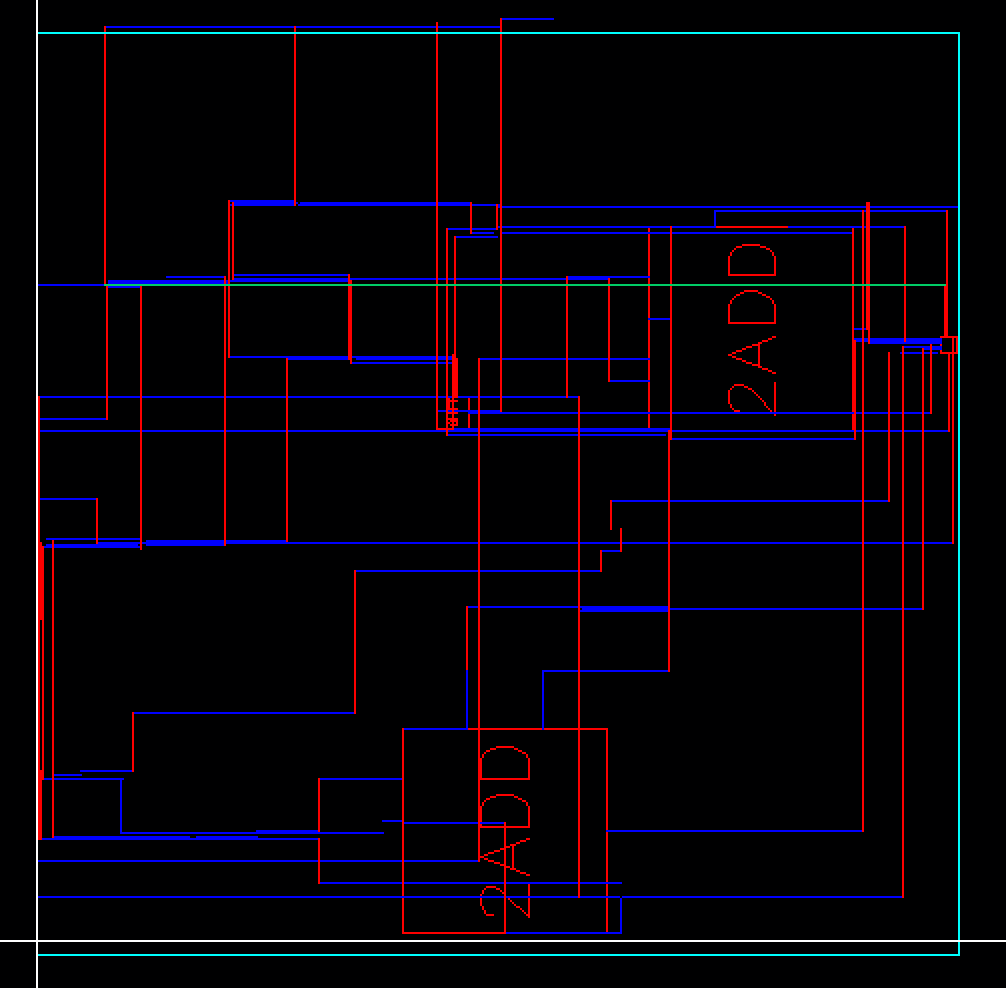
\includegraphics[scale=0.5]{masterlayout.png} \\
  \newline \newline
  As you can see, the adder is easily the largest module in the layout. 
  \newline \newline
  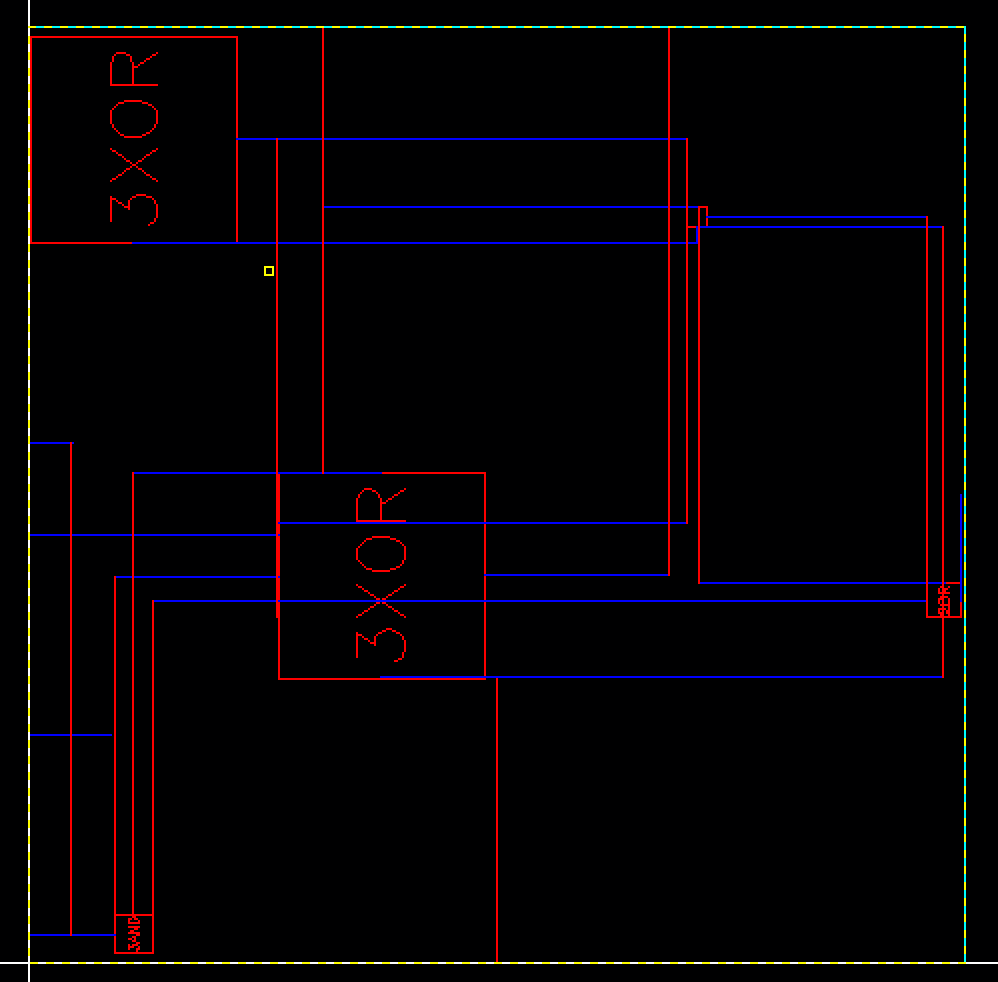
\includegraphics[scale=0.5]{adderlayout.png} \\
  \newline \newline
  Which, in turn, has XOR's and AND's. Obviously, the XOR is bigger than the AND.
  \newline \newline
  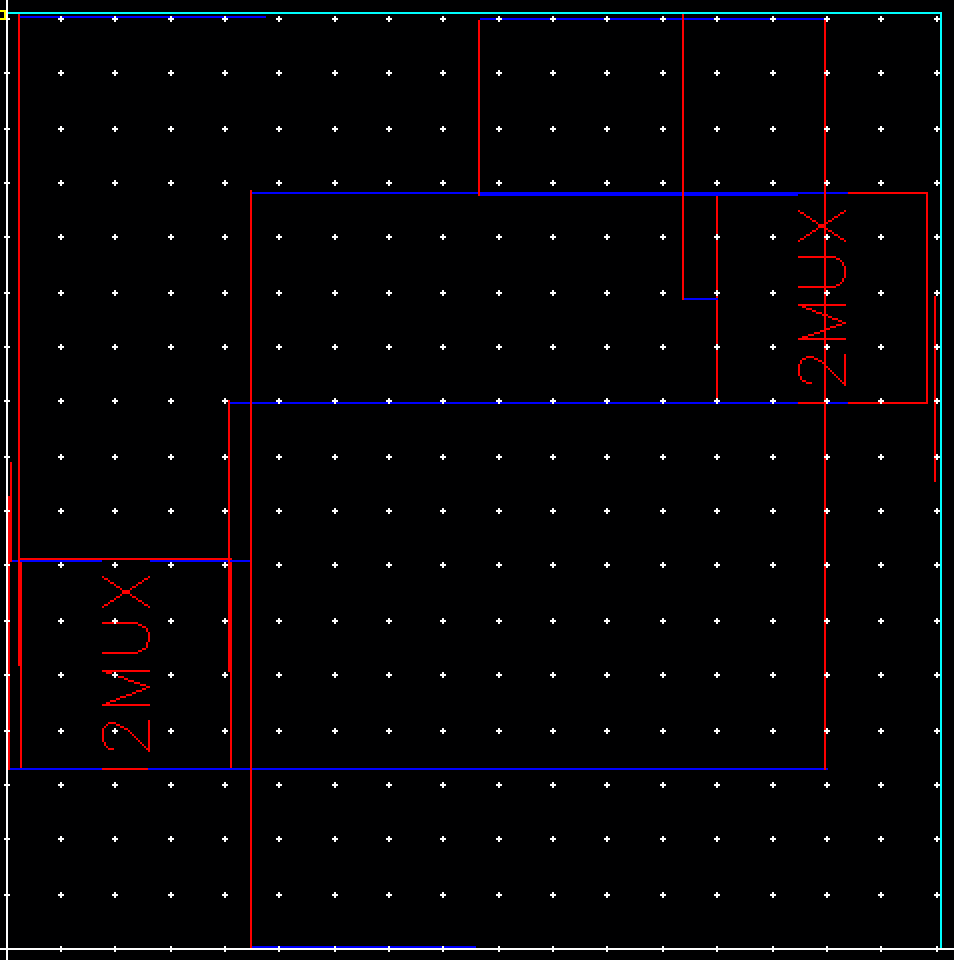
\includegraphics[scale=0.5]{shiftlayout.png} \\
  \newline \newline
  The shifter, made of 2MUX's is relatively straightforward when moving from schematic to layout.
  \newline \newline
  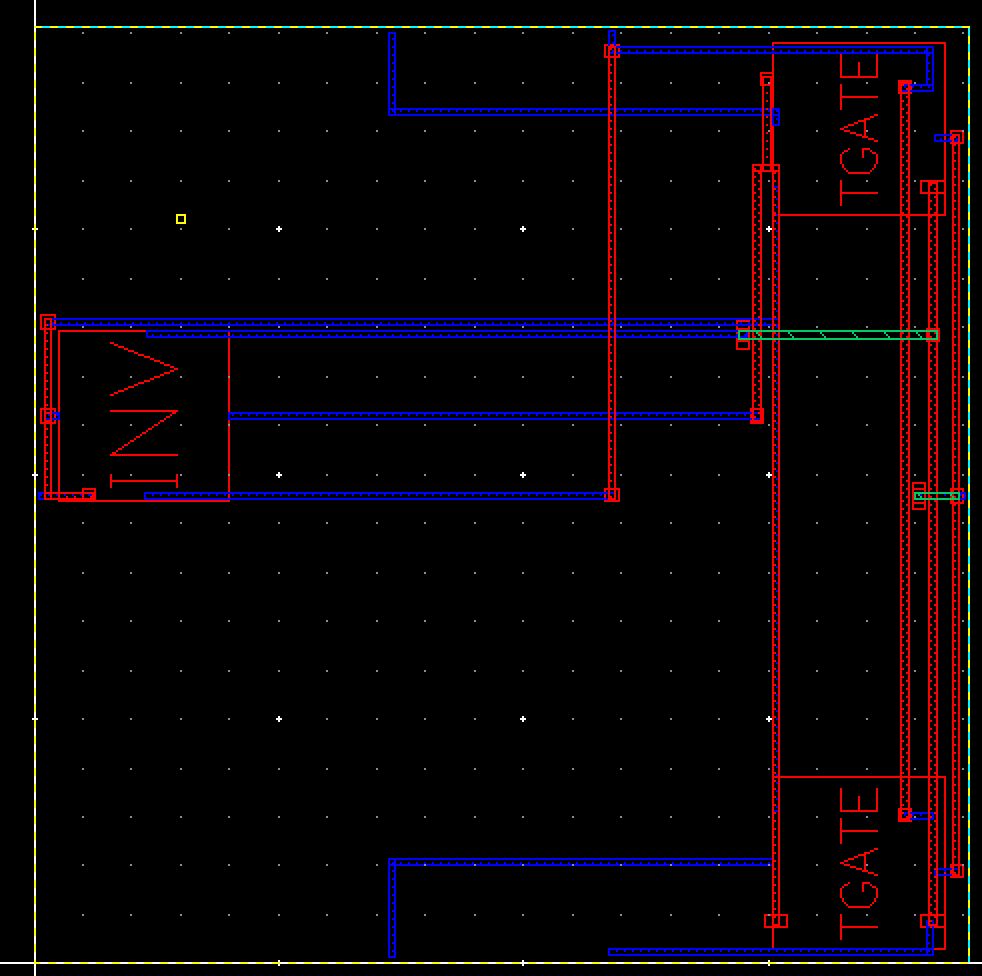
\includegraphics[scale=0.5]{muxlayout.png} \\
  \newline \newline
  And the mux has 2TGATE's and an INVERTER. Simple, straightforward compared to the master.
  \newline \newline
  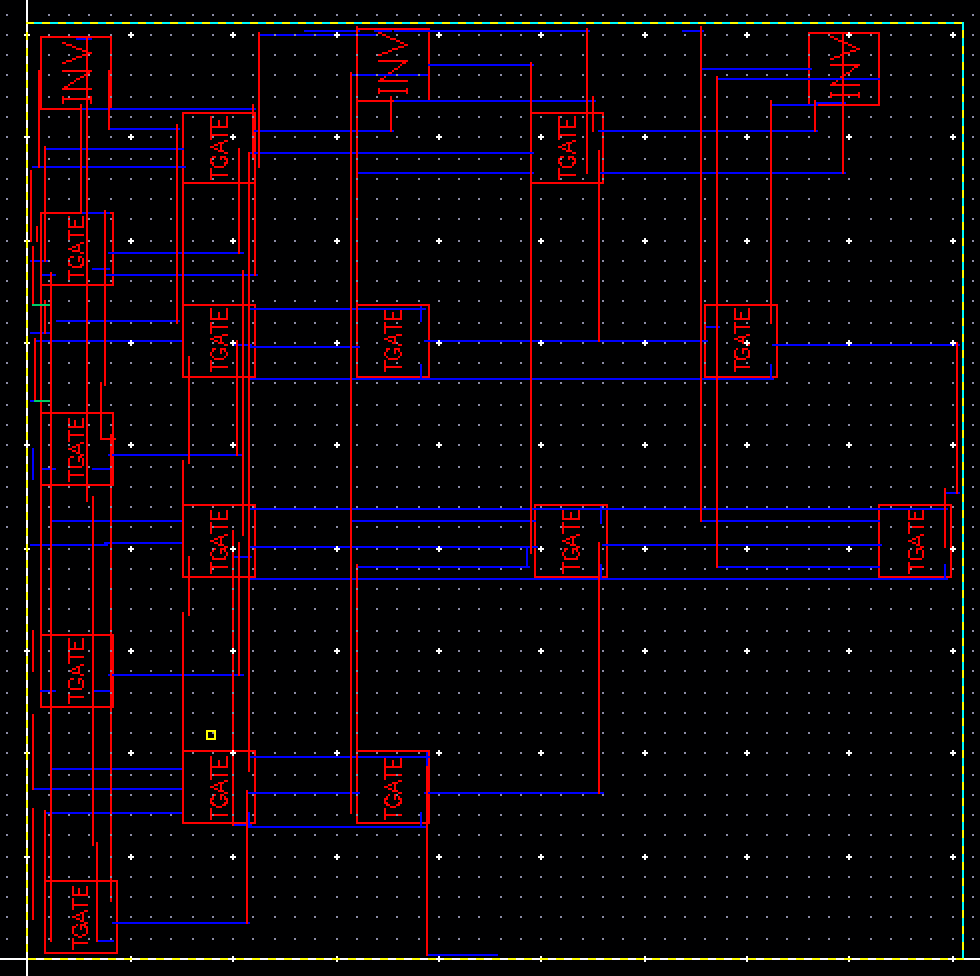
\includegraphics[scale=0.5]{8muxlayout.png} \\
  \newline \newline
  The 8 mux wasn't straightforward, however. But it's layout was repetitive, which in its very nature 
  made mistakes easier to catch.
  \newline \newline
  All in all, the only headache came when, for no reason, the automatic routing would simply not the
  Vdd and Gnd connections, or wire the body of the transistors to the wrong placed. 
  \newline \newline
	\textbf{A Look at the Adder Delay}
  \newline \newline
  For the adder, as mentioned previously we used the carry-lookahead methodology to implement it.
  From there, we took two measurements: one of the propagation delay on the ouput, and the other on
  the propagation delay of the carry-out. The following graphics demonstrate the delays:
  \newline \newline
  \newline \newline
  Delay of sum on the adder:
  \newline \newline
  \newline \newline
  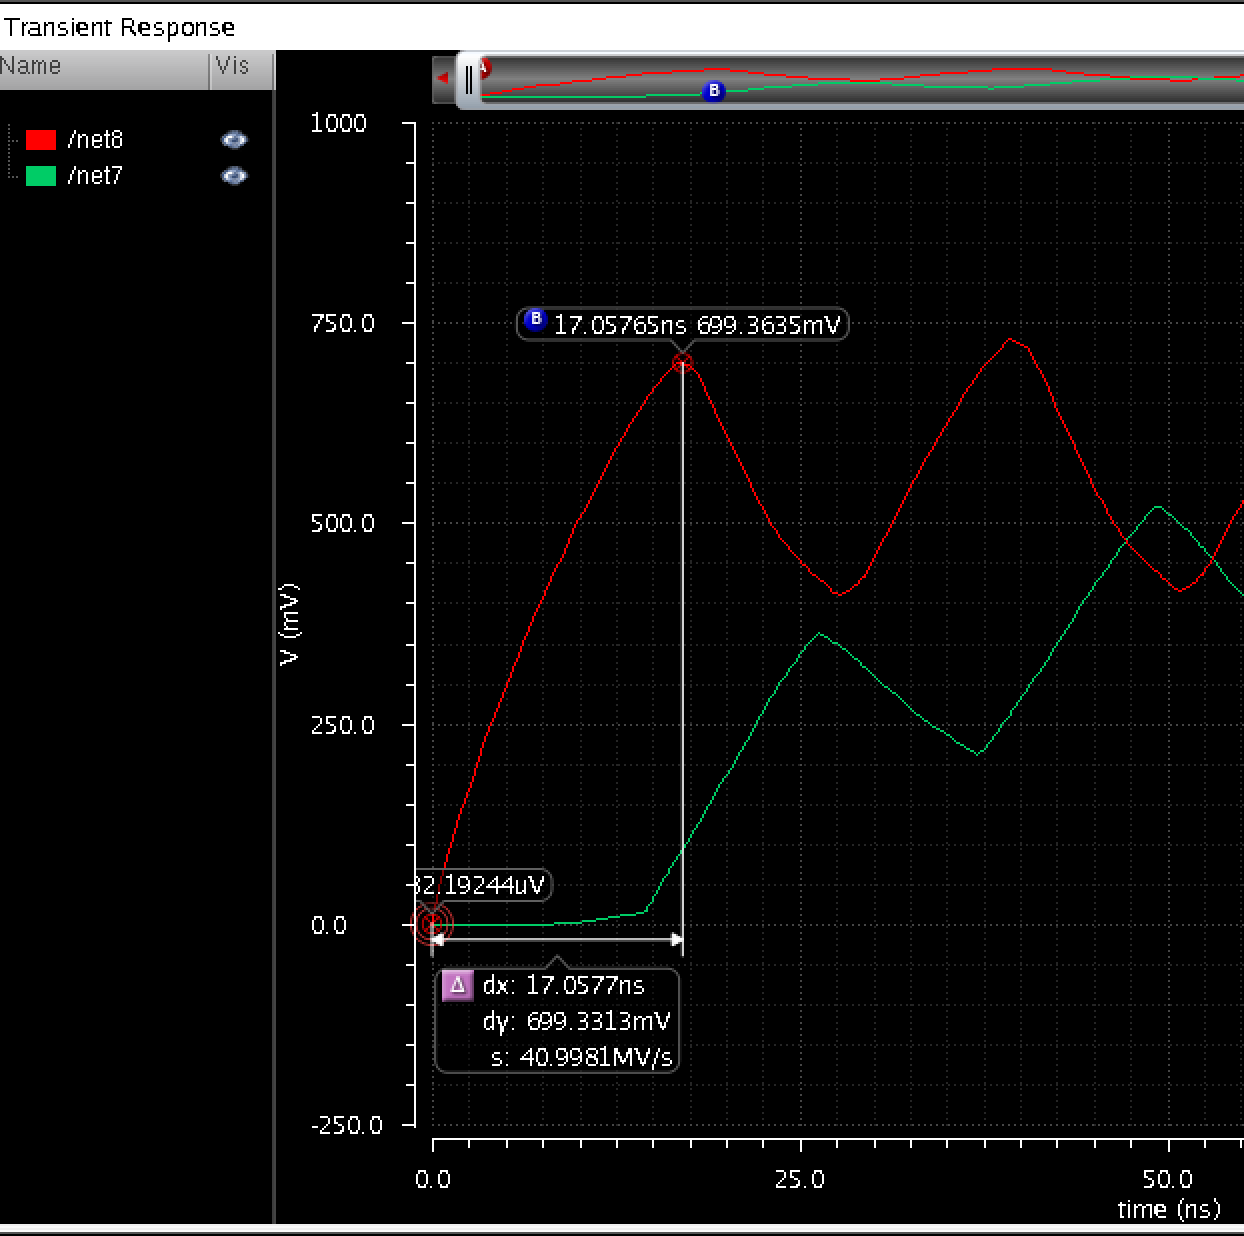
\includegraphics[scale=0.4]{delaysum.png} 
  \newline \newline
  Delay of cout on the adder:
  \newline
  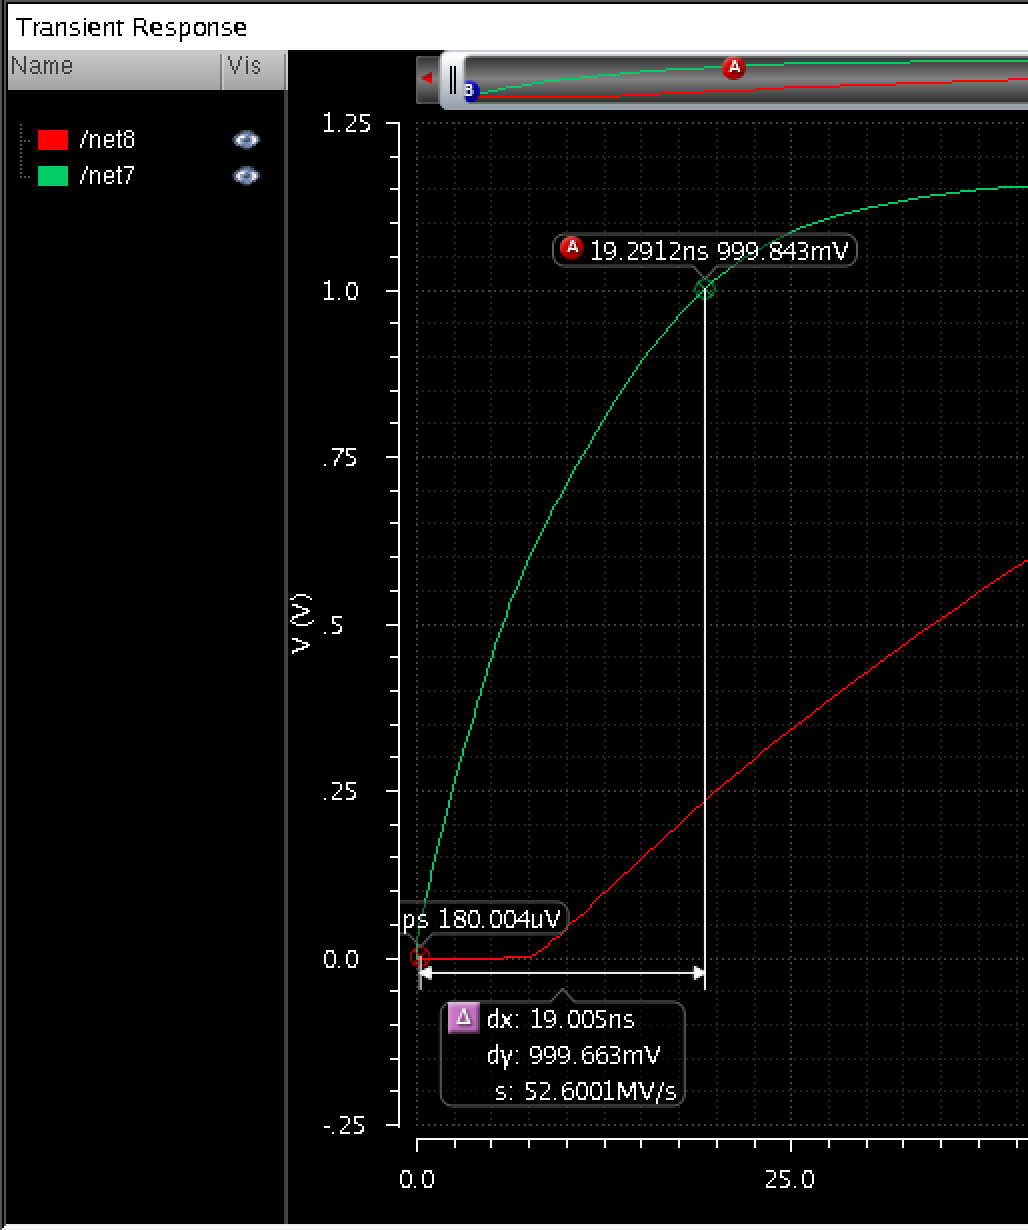
\includegraphics[scale=0.4]{delaycout.png} \\
  \newline \newline
  As the graphs portray, the sum takes about 17.057 ns and the cout takes about 19.29 ns. We can 
  set the high voltage cutoff to be slightly lower to about 0.9 V to bring that number down to roughly
  17.042 ns. This number is a bit higher than we expected. We attempted fix that by doing better transistors sizing to 
  pass the constants necessary for the Cout to come faster; however, due to timing constraints and lack of access
  to Cadence during critical times, we were unable to properly implement and more importantly measure the delay
  generated by doing so. Currently, they are all of uniform size (PMOS width = 2* NMOS width), which of course 
  is not ideal and was planned to be fixed once we learned about benefits non-unifrom or unity-driven sizing. But 
  once again, due timing constraints and the poor reliability of the Cadence software, this is the best we have 
  in our current version. Please understand and know that we genuinely knew this would have reduced delay by
  several nanoseconds. There is, however, the observation that this is the time it takes to \textbf{generate} a Cout
  rather than propagate, and thus the total delay through the whole circuit will be much, much less than 16 times
  this value.
  \newline \newline
	\textbf{Energy Consumption}
  \newline \newline
  The dynamic energy consumption is a factor of the amount of switching done by the transistors due
  the work being done. Using the Calculator in Cadence, the graphic below demonstrates that energy 
  consumption (and power, for that matter).
  \newline \newline
  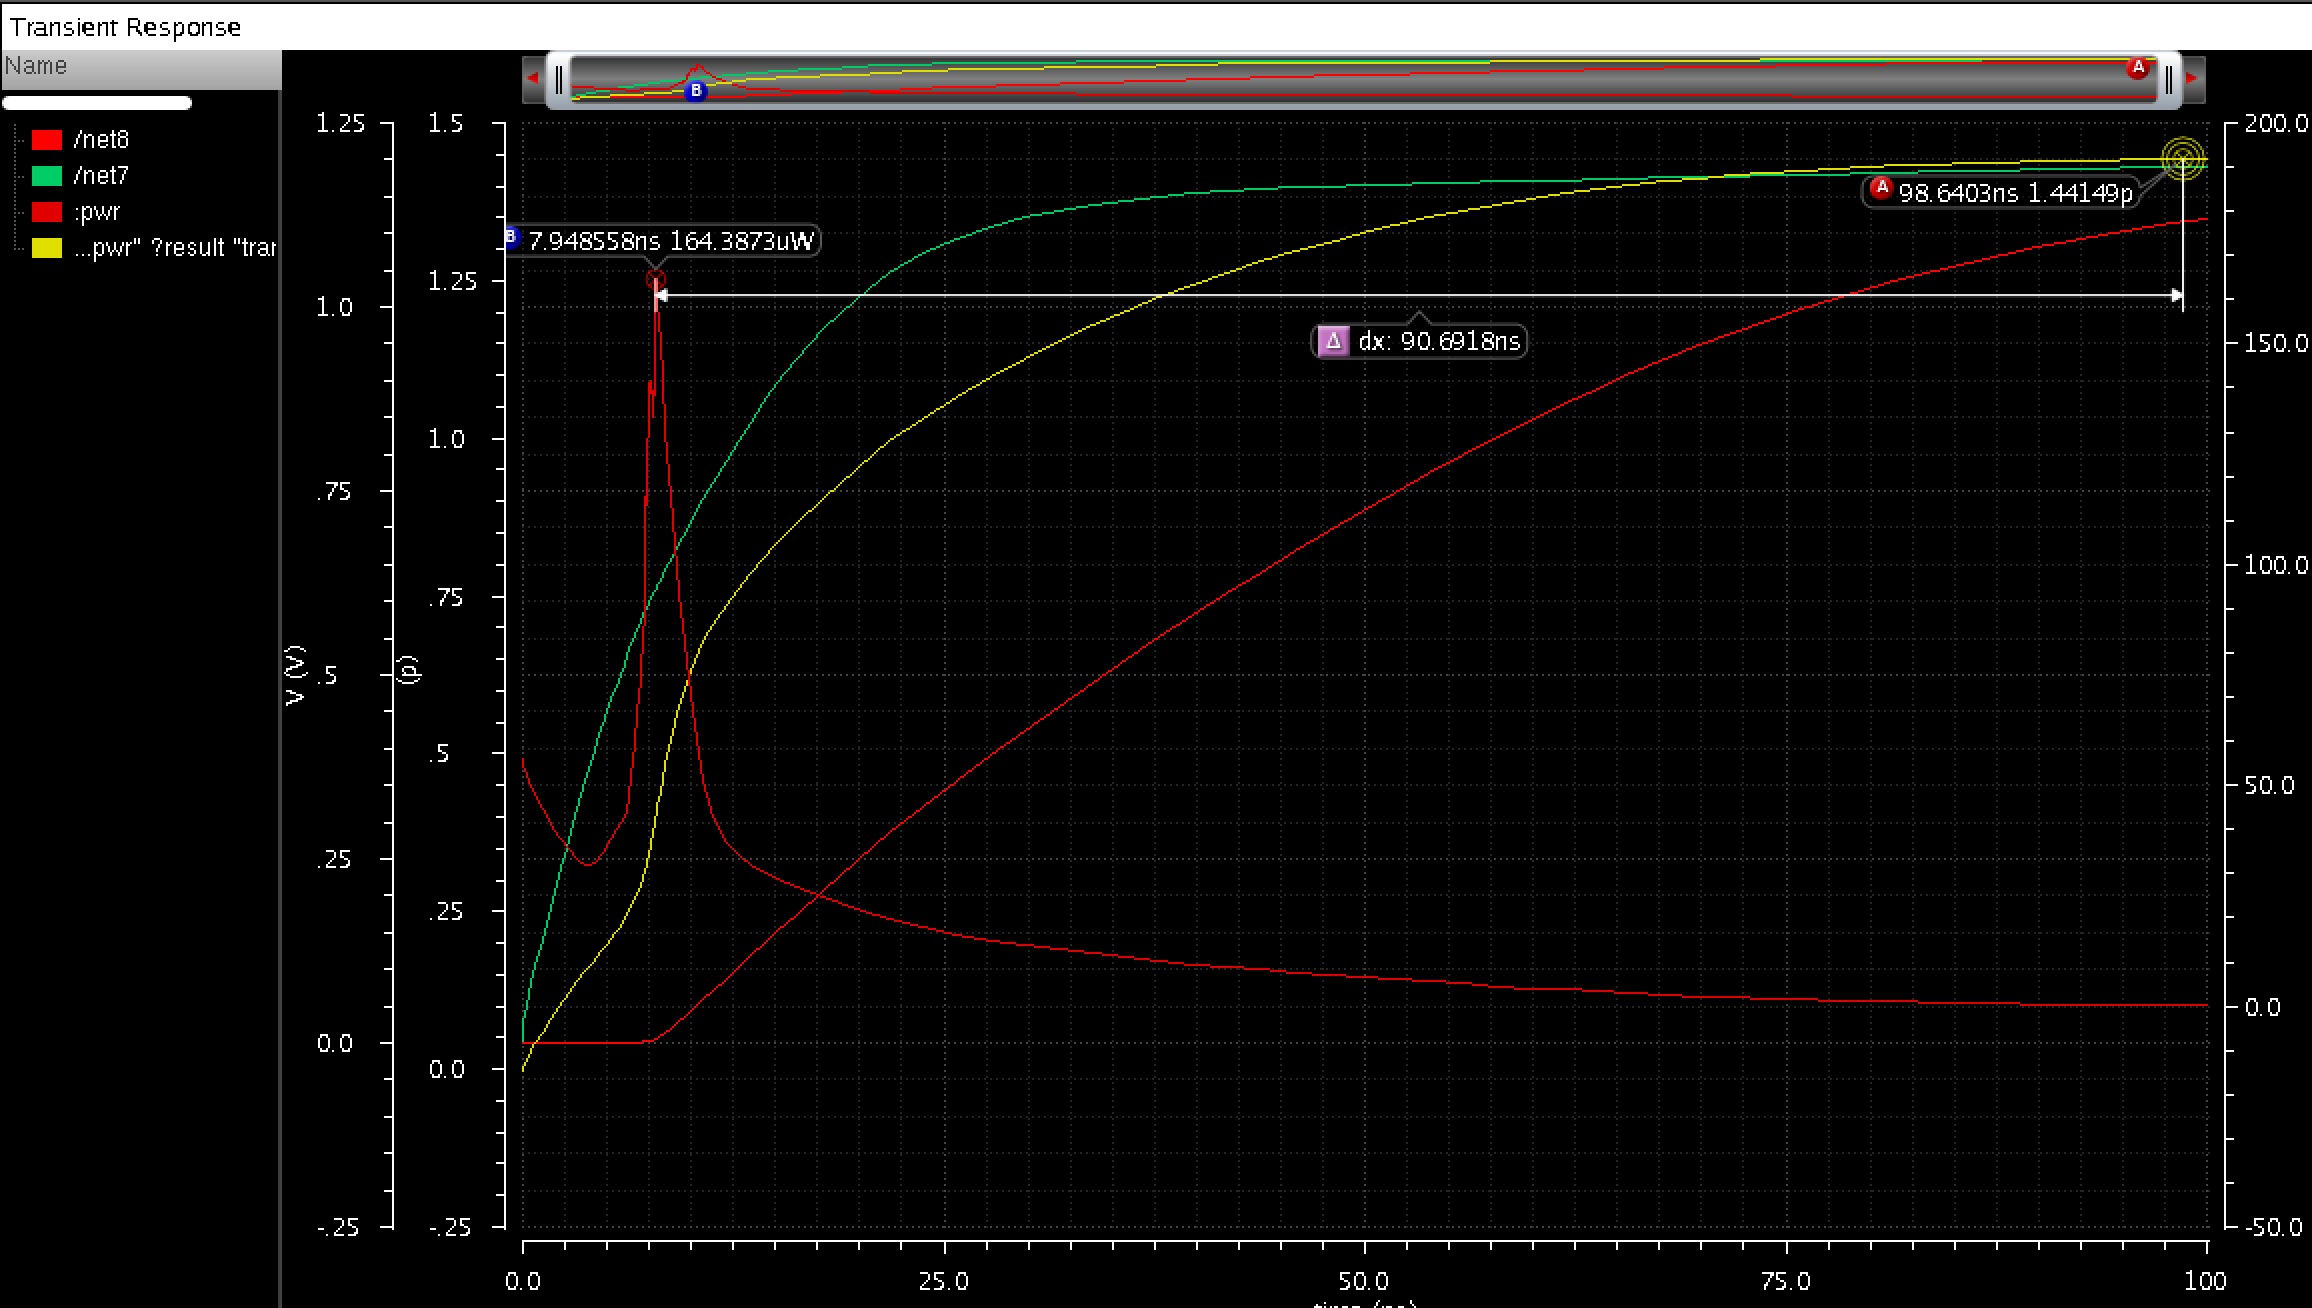
\includegraphics[scale=0.4]{energy.png} \\
  \newline \newline
  The peak power output was about 164 $\mu$ W, and the dynamic energy consumption is about 1.44 pJ.
  This is representative of a majority of the paths in our circuit. If anything, only the subtract
  instruction will incur a slightly larger energy consumption. Other than that, the energy is upper-bounded
  by this, since use of the adder in the ALU is the most expensive procedure.
    \newline \newline
	\textbf{Energy Delay Product Computation}
  \newline \newline
  Our approach to compute the worst case energy product delay for the full ALU add operation was to first compute
  the product for our bit slice layout and then extend that number to accommodate for 16 bits. As we computed the
  dynamic energy consumption of the add operation turned out to be 1.44 pJ, while the delay of the Cout of the 
  add operation was roughly about 17.042 ns (generate). We believe that the Cout operation will be the 
  limiting factor in the scenario of the worst case delay since all generates, in the worst case, will be computed 
  as 0 while all propagates will be computed as 1. In other words, each bit slice will need to pass the Cin to the Cout
  and while factoring in the Cin for the sum operation. The sum operations, however, have a lot of time to compute
  and are thus not the critical path. The propagate signal is a 3 bit XOR operation and takes roughly 614 ps. This
  computation is done in parallel for all 16 bits starting at time t = 0, which is less time than it takes to generate
  the first Cout on bit slice 0. The propagation delay is thus the delay through a 2 input AND and a 2 input OR, 
  which is roughly 209 ps and 250 ps respectively. Therefore the delay from Cin to Cout is 209 + 250 ps = 459 ps. 
  Additionally, the cost of incorporating Cin into the sum is a roughly 5.14 ns delay (this matters for the most 
  significant bit). Therefore, the total delay in the worst case situation for the 16 bit add operation is:
  \newline
  \[17.042 ns + 14*459 ps + 5.14 ns = 28.608 ns\]
  \newline
  The energy consumption is roughly the same per bit slice (1.44 pJ). The total energy consumption is thus:
  \newline
  \[16*1.44 pJ = 23.04 pJ\]
  \newline
  Therefore, the worst case energy product delay is:
  \newline
  \[28.608 * 23.04 = \boxed{659.128}\]
  
 \section{}
 
 \textbf{Extending to Verilog}
 \newline \newline
 For the Verilog bit slice implementation as well as its corresponding testbench, please observe the attached files.
 All delays from the layout design were incorporated directly from the layout design into the module implementation
 to ensure an "as-accurate-as-possible" simulation.
 
  \section{}
 
 \textbf{ALU Implementation}
 \newline \newline
The full 16 bit ALU was implemented by wiring 16 different bit slice instantiations following a reasonably simple 
naming convention. All dangling input and output wires from the bit slice implementation were attached to their 
appropriate wires in full ALU Verilog instantiation as well, and all operations work as expected. To view the 
implementation, please see the attached Verilog file. 
 \newline \newline
 \textbf{Datapath Implementation}
 \newline \newline
The full datapath was implemented using the register instances specified in the project guidelines and contains
an instantiation of the 16 bit ALU. The MUX gates are simulated via a series of input signals and assignment / if
statements to ensure that only the proper input is written to the proper register or sent to the ALU. The OpCodes
are collected and translated into the appropriate datapath signals by a module called the Control Block; the datapath 
itself only follows the signals it is provided and is not responsible for any kind of serialization or deserialization. It
uses the same clock as the Control Block as well. The OpCode input is merely meant to be passed in to the ALU
if necessary. For the full module and its corresponding testbench, please see the attached Verilog files. 
 \newline \newline
\textbf{Remaining Components}
\newline \newline
Structure:
\newline \newline
The layout is as follows, from top-bottom
\begin{enumerate}
	\item main.v OR demonstrate.v (explained later)
	\item control.v
	\item datapath.v
	\item ALU.v
	\item bitslice.v
	\item adder.v/subtractor.v
\end{enumerate}
Main Module:
\newline \newline
**Both main.v and demonstrate.v have testbenches, tbMain.v and tbDemonstrate.v** 
\newline \newline
For testing purposes, *main.v* should be considered the "main" module. It is left empty (other than connected to our controller), and its testbench merely shows how to multiply two numbers together.
\newline \newline
**HOWEVER**
\newline \newline
demonstrate.v has a nicer way of demonstrating the correctness of the routines. It has built in tasks for add, multiply, right shift, and two's complement. Those demonstrate basically all the required procedures for this protocol. *All the testbench does is provide you a place to input an X and Y*. For any new X and Y, demonstrate.v reruns all these tasks and outputs the monitor for them as well as the final values in a very human readable form.  Here is an image providing an example. You can always se the original inputs X and Y and what the results for each task are:
![add shift complement](demonstrate1.png)
![multiply](demonstrate2.png)
\newline \newline
**We highly suggest you use demonstrate.v and tbDemonstrate.v first to get a feel for how easy it should be to test that our main functions are working**. 
Only after seeing it run a couple of times, and after having read the section below on how to use our opcodes, should you add stuff to tbMain.v for testing the main fucntion
\newline \newline
OPCODE BREAKDOWN:
\newline \newline
Passed to the control block is a 12 bit opcode. There are 8 prefix bits and 4 ALU bits.
The meaning of each are as follows
\newline \newline
M1  M2  M3  M4  M5  M5  RegOut RegOut ALU ALU ALU ALU
\newline \newline
M1 through M5 are the selector bits for each of the 5 MUX's (M5 has two bits for 3 inputs)
\newline \newline
RegOut indicates which register (X,Y,Z which correspond to Aout,Bout,Cout in the diagram provided with the spec) to write to (2 bits are needed for 3 outputs)
\newline \newline
ALU indicates the 4 bit opcode for the ALU
\newline \newline
If the last four bits are an actual operation in the ALU, then the following decoding is used:
\begin{enumerate}
	\item Observe M3 to choose which register, A or B, to read from.
	\item Observe M4 to choose to either read from reg C or from output registers.
	\item If M4 is reading from feedback, observe M5 to see which output register to read from.
	\item Compute ALU function using ALU opcode, and observe RegOut to see which register to store the data in.
\end{enumerate}
If the last four bits are a datapth operation (Load into A/B/C) then the following decoding is used:
\begin{enumerate}
	\item Observe opcode. If it is Load A/B, observe M1 to either read X or read from feedback.
	\item If M1 indicates to observe from feedback, observe M5 to see which output register to read from.
	\item If opcode indicates to Load C, observe M2 to either read Y or read from feedback.
	\item If M2 indicates to observe from feedback, observe M5 to see which output register to read from.
\end{enumerate}
For example, if we wanted to first store something from Z into B, the following opcode would handle it (spaced out for convenience):
\newline \newline
1  0  0  0  1  0  0      0      1   0   1   1
M1 M2 M3 M4 M5 M5 RegOut RegOut ALU ALU ALU ALU
\newline \newline
This means that mux-1 choses to receive input from feedback. Mux 2-4 we don't care about since the operation doesn't involve them. Mux-5 with 10 means to read from Z. RegOut is 0 0 because we are not writing to any output register. Finally, ALU code 1011 means load into B.
\newline \newline
Then, if we want to calculate the bitwise and B with what is currently in Y and store it in Z, the following opcode would handle it:
\newline \newline
0  0  1  1  0  1  1      0      0   1   1   0
M1 M2 M3 M4 M5 M5 RegOut RegOut ALU ALU ALU ALU
\newline \newline
Mux-1,2 are don't cares. Mux-3 being 1 means to read from register B, and Mux-4 being 1 means to read from feeback (from output registers). Mux-5 being 01 means to read from output register Y, and RegOut of 10 means to write to register Z. ALU opcode 0110 indicates to perform the bitwise \& of the two operators. 
\newline \newline
That's all there is to it. This same documentation (minus the examples) is in control.v
\newline \newline
Final Notes:
\begin{enumerate}
	\item For the last few Verilog modules, they were developed locally on a Mac using [Icarus Verilog](http://iverilog.icarus.com/). It, 
	for all intensive purposes, should work in ModelSim as well. However, if it doesn't work, please contact Joraaver Chahal, and don't 
	immediately deduct points please. The connection was too slow and becoming a realy pain to work on ModelSim via ssh, and I took 
	the initative to find a local development environment dad the did the trick. Frankly, I think Icarus Verilog does a great, minimalist job 
	for compiling and testing Verilog tools. It dropped support of a synthesis tool, but other open source synthesis tools exist for 
	FPGA's, so that's not a problem.

	\item I won't say this project was fun. It was a huge time commitment that I felt could have been made more manageable. However, 
	as I always, we did learn alot about the full process in terms of laying out the ALU's bitslice and incorporating the extracted delays 
	into the simulation, so there's always that.
\end{enumerate}
\end {document}


